%---------------------------preamble--------------------------------------
%-------------------------------------------------------------------------
%--------------Preamble----------------------------------------------------
%compile this package with pdflatex
\documentclass[10pt]{beamer} % default
%\documentclass[10pt,aspectratio=169]{beamer} % default
%\documentclass[draft,10pt,aspectratio=169]{beamer} % draft
%\documentclass[handout,10pt,aspectratio=169]{beamer} % handout
%-------------------------------------------------------------------------
% my def
\definecolor{tuhh_darkcyan}{rgb}{.09,0.39,.42}
\def\LBOX{\fbox{\begin{minipage}[c][.4cm][c]{.5cm}%
  \center \large \phantom{1} \qquad\end{minipage}}}
\newcommand\BOXWF[1]{\fbox{\begin{minipage}[c][.4cm][c]{.5cm}%
  \center \large {#1}\end{minipage}}}
% my def
%-------------------------------------------------------------------------
%
\usepackage{amsfonts}
\usepackage{amssymb}
\usepackage[ngerman]{babel}
\usepackage{ulem}
\normalem
\usepackage{bookmark}
\usepackage{apalike}
%%%%%%%%%%%%%%%%%%%%%%%%%%%%%%%%%%%%%%%%%%%%%%%%%%%%%%%%%%%%%%%%%%%%%%%%%%%%%%%
% Definitions
%%%%%%%%%%%%%%%%%%%%%%%%%%%%%%%%%%%%%%%%%%%%%%%%%%%%%%%%%%%%%%%%%%%%%%%%%%%%%%%
%
% Colors:
  \definecolor{myalgcolor}{rgb}{1.0,1.0,0.5}
  \definecolor{myred}{rgb}{1.0,0.0,0.0}
  \definecolor{myyellow}{rgb}{1.0,1.0,0.5}
  \definecolor{mygray}{gray}{0.55}
  \definecolor{mycyan}{rgb}{.0,.8,1.0}
  \definecolor{blau}{rgb}{.5,.5,1.0}
  \definecolor{myerror}{rgb}{1.0,0.0,0.5}
  \definecolor{myerron}{rgb}{0.4,0.0,0.6}
\newcommand{\error}[1]{\textcolor{myerror}{{}#1{}}}
\newcommand{\erron}[1]{\textcolor{myerron}{{}#1{}}}
\newcommand{\backupbegin}{
   \newcounter{framenumberappendix}
   \setcounter{framenumberappendix}{\value{framenumber}}
}
\newcommand{\backupend}{
   \addtocounter{framenumberappendix}{-\value{framenumber}}
   \addtocounter{framenumber}{\value{framenumberappendix}}
}
\DeclareMathOperator{\diag}{\mathsf{diag}}
\DeclareMathOperator{\argmin}{\mathsf{argmin}}
\DeclareMathOperator{\codim}{\mathsf{codim}}
\DeclareMathOperator{\Rang}{\mathsf{Rang}}
\DeclareMathOperator{\zeros}{\mathsf{zeros}}
\newcommand{\bfnu}{\boldsymbol{\nu}}
\newcommand{\bfhatnu}{\boldsymbol{\widehat{\nu}}}
\newcommand{\bfchecknu}{\boldsymbol{\check{\nu}}}
\DeclareMathOperator{\sut}{\mathsf{sut}}
\DeclareMathOperator{\tril}{\mathsf{tril}}
\DeclareMathOperator{\triu}{\mathsf{triu}}
\renewcommand{\diag}{\mathsf{diag}}
\DeclareMathOperator{\diagm}{\mathsf{diag}}
\DeclareMathOperator{\trace}{\mathsf{trace}}
\DeclareMathOperator{\sign}{\mathsf{sign}}
%
%%%%%%%%%%%%%%%%%%%%%%%%%%%%%%%%%%%%%%%%%%%%%%%%%%%%%%%%%%%%%%%%%%%%%%%%%%%%%%%
% Definitions added by Rustam Magomedov
%%%%%%%%%%%%%%%%%%%%%%%%%%%%%%%%%%%%%%%%%%%%%%%%%%%%%%%%%%%%%%%%%%%%%%%%%%%%%%%
%% my own stuff
%%
%% definition of perlis mathclap etcpp.
%%
% For comparison, the existing overlap macros:
% \def\llap#1{\hbox to 0pt{\hss#1}}
% \def\rlap#1{\hbox to 0pt{#1\hss}}
\def\clap#1{\hbox to 0pt{\hss#1\hss}}
\def\mathllap{\mathpalette\mathllapinternal}
\def\mathrlap{\mathpalette\mathrlapinternal}
\def\mathclap{\mathpalette\mathclapinternal}
\def\mathllapinternal#1#2{%
  \llap{$\mathsurround=0pt#1{#2}$}}
\def\mathrlapinternal#1#2{%
  \rlap{$\mathsurround=0pt#1{#2}$}}
\def\mathclapinternal#1#2{%
  \clap{$\mathsurround=0pt#1{#2}$}}
%%
%% end of perlis stuff
%%
%%
%% definition of inverse diagonal dots (iddots)
%%
\makeatletter
\def\iddots{\mathinner{\mkern1mu\raise\p@%
    \hbox{.}\mkern2mu\raise4\p@\hbox{.}\mkern2mu%
    \raise7\p@\vbox{\kern7\p@\hbox{.}}\mkern1mu}}
\makeatother
%%%\def\ddots{\mathinner{\mkern1mu\raise7\p@\vbox%
%%%{\kern7\p@\hbox{.}} \mkern2mu\raise4\p@\hbox{.}%
%%%\mkern2mu\raise\p@\hbox{.}\mkern1mu}}
%
% TIME OF DAY (Nelson H. F. Beebe :-)
%
\newcount\hh
\newcount\mm
\mm=\time
\hh=\time
\divide\hh by 60
\divide\mm by 60
\multiply\mm by 60
\mm=-\mm
\advance\mm by \time
\def\hhmm{\number\hh:\ifnum\mm<10{}0\fi\number\mm}
%
% Use it like this in a LaTeX document:
%
%        \date{\today{ }\hhmm}
%
%%%%%%%%%%%%%%%%%%%%%%%%%%%%%%%%%%%%%%%%%%%%%%%%%%%%%%%%%%%%%%%
%%%
%%% kleiner Hack, um Einträge in Matrizen anders auszurichten
%%%
%%%%%%%%%%%%%%%%%%%%%%%%%%%%%%%%%%%%%%%%%%%%%%%%%%%%%%%%%%%%%%%
\makeatletter
\renewcommand*\env@matrix[1][*\c@MaxMatrixCols c]{%
  \hskip -\arraycolsep
  \let\@ifnextchar\new@ifnextchar
  \array{#1}}
\makeatother
%%%%%%%%%%%%%%%%%%%%%%%%%%%%%%%%%%%%%%%%%%%%%%%%%%%%%%%%%%%%%%%
%%%
%%% Wir wollen Matlab-Beispielprogramme einbinden
%%%
%%%%%%%%%%%%%%%%%%%%%%%%%%%%%%%%%%%%%%%%%%%%%%%%%%%%%%%%%%%%%%%
\usepackage{listings}
\definecolor{hellgrau}{rgb}{0.90,0.90,0.90}
\definecolor{commentcol}{rgb}{0.0823,.4902,0.0}
\lstset{language=Matlab,
        basicstyle={\footnotesize\ttfamily},
        keywordstyle={\sffamily\bfseries},
        tabsize=2,
        escapechar=\#,
        numbers=left,
        numberstyle=\tt,
        stepnumber=1,
        numbersep=7pt,
        breaklines=true,
        frame=single,
        frameround=ffff,
        commentstyle=\color{commentcol},
        backgroundcolor=\color{hellgrau}
}
\usepackage{algorithmic}
\renewcommand{\algorithmiccomment}[2]{\hfill\rlap{\texttt{\%
      #1}}\phantom{\texttt{\% #2}}}
\renewcommand{\algorithmicrequire}{\textsc{Eingabe:}}
\renewcommand{\algorithmicensure}{\textsc{Ausgabe:}}
\usepackage{algorithm}
\floatname{algorithm}{Algorithmus}

\mode<presentation>
{
  \usetheme{ABMATH}
  \useinnertheme{default}
  \setbeamercovered{invisible}
  \usefonttheme[onlymath]{serif}
  \setbeamertemplate{items}[circle]
  \setbeamertemplate{sections/subsections in toc}[default]
  \setbeamercolor*{author in head/foot}{parent=palette secondary}
}
\setbeamerfont{quote}{shape=\upshape}
\usepackage{pgf}
\usepackage[utf8]{inputenc}
\usepackage[T1]{fontenc}
\usepackage{times}
\usepackage{graphicx}
\usepackage{pifont}
\usepackage{colortbl}
\usepackage{xmpmulti}
\usepackage{multimedia}
\usepackage{pdfpages}
\usepackage{tikz}
\usepackage{pgfplots}

\newcommand{\bfA}{{\mathbf A}}
\newcommand{\bfB}{{\mathbf B}}
\newcommand{\bfC}{{\mathbf C}}
\newcommand{\bfD}{{\mathbf D}}
\newcommand{\bfE}{{\mathbf E}}
\newcommand{\bfF}{{\mathbf F}}
\newcommand{\bfG}{{\mathbf G}}
\newcommand{\bfH}{{\mathbf H}}
\newcommand{\bfI}{{\mathbf I}}
\newcommand{\bfJ}{{\mathbf J}}
\newcommand{\bfK}{{\mathbf K}}
\newcommand{\bfL}{{\mathbf L}}
\newcommand{\bfM}{{\mathbf M}}
\newcommand{\bfN}{{\mathbf N}}
\newcommand{\bfO}{{\mathbf O}}
\newcommand{\bfP}{{\mathbf P}}
\newcommand{\bfQ}{{\mathbf Q}}
\newcommand{\bfR}{{\mathbf R}}
\newcommand{\bfS}{{\mathbf S}}
\newcommand{\bfT}{{\mathbf T}}
\newcommand{\bfU}{{\mathbf U}}
\newcommand{\bfV}{{\mathbf V}}
\newcommand{\bfW}{{\mathbf W}}
\newcommand{\bfX}{{\mathbf X}}
\newcommand{\bfY}{{\mathbf Y}}
\newcommand{\bfZ}{{\mathbf Z}}
\newcommand{\bfa}{{\mathbf a}}
\newcommand{\bfb}{{\mathbf b}}
\newcommand{\bfc}{{\mathbf c}}
\newcommand{\bfd}{{\mathbf d}}
\newcommand{\bfe}{{\mathbf e}}
\newcommand{\bff}{{\mathbf f}}
\newcommand{\bfg}{{\mathbf g}}
\newcommand{\bfh}{{\mathbf h}}
\newcommand{\bfi}{{\mathbf i}}
\newcommand{\bfj}{{\mathbf j}}
\newcommand{\bfk}{{\mathbf k}}
\newcommand{\bfl}{{\mathbf l}}
\newcommand{\bfm}{{\mathbf m}}
\newcommand{\bfn}{{\mathbf n}}
\newcommand{\bfo}{{\mathbf o}}
\newcommand{\bfp}{{\mathbf p}}
\newcommand{\bfq}{{\mathbf q}}
\newcommand{\bfr}{{\mathbf r}}
\newcommand{\bfs}{{\mathbf s}}
\newcommand{\bft}{{\mathbf t}}
\newcommand{\bfu}{{\mathbf u}}
\newcommand{\bfv}{{\mathbf v}}
\newcommand{\bfw}{{\mathbf w}}
\newcommand{\bfx}{{\mathbf x}}
\newcommand{\bfy}{{\mathbf y}}
\newcommand{\bfz}{{\mathbf z}}
\newcommand{\bfell}{{\boldsymbol\ell}}
\newcommand{\bfSigma}{{\boldsymbol\Sigma}}
\newcommand{\DEF}{:=}
\newcommand{\FED}{=:}
\newcommand{\DEFM}[1]{\textcolor{red}{#1}}
\newcommand{\T}{\mathsf{T}}
\renewcommand{\H}{\mathsf{H}}
\newcommand{\Span}{\mathop{\mathsf{span}}}
\newcommand{\spec}{\mathop{\mathsf{spec}}}

%%% thanks, Nick Higham :)
\setbeamertemplate{navigation symbols}{}

\usepackage[absolute,overlay]{textpos}











%%%%%%%%%%%%%%%%%%%%%%%%%%%%%%%%%%%%%%%%%%%%%%%%%%%%%%%%%%%%%%
%%%%%%%%%%%% my own packages %%%%%%%%%%%%%%%%%%%%%%%%%%%%%%%%%
%%%%%%%%%%%%%%%%%%%%%%%%%%%%%%%%%%%%%%%%%%%%%%%%%%%%%%%%%%%%%%

\title[Pivotisierung]%
{Gaußsches Eliminationsverfahren mit Pivotisierung}

\author[Rustam Magomedov]%
{%
	{Rustam Magomedov}\break
  \footnotesize{\href{mailto:rustam.magomedov@tuhh.de}%
                {rustam.magomedov@tuhh.de}}%
}

\titlegraphic{%
  \includegraphics[height=.15\textheight]%
    {pics/TUHH_de}%
}

% \institute{\href{https://www.mat.tuhh.de/}{%
%             Institut für Mathematik}\\
%             Lehrstuhl Numerische Mathematik\\
%            \href{https://www.tuhh.de/}{%
%             Technische Universität Hamburg}%
% }

\date[2017-05-08]{\footnotesize{8. May 2017}}

\AtBeginSubsection[]
{
  \begin{frame}<beamer>
    \frametitle{Übersicht}
    \tableofcontents[currentsection,currentsubsection]
%    \tableofcontents[currentsection]
  \end{frame}
}
% \AtBeginSection[]
% {
%   \begin{frame}<beamer>
%     \frametitle{Übersicht}
% %    \tableofcontents[currentsection,currentsubsection]
%     \tableofcontents[currentsection]
%   \end{frame}
% }
%---------------------------preamble-----------------------------------
\hypersetup{%
  pdftitle     = {},
  pdfsubject   = {},
  pdfkeywords  = {},
  pdfauthor    = {\textcopyright\ Rustam Magomedov, May 2017},
  % pdfpagemode  = FullScreen
%  colorlinks = true,
%  linkcolor = ,
%  urlcolor = blue,
}
\usetikzlibrary{matrix,fit}





%%%%%%%%%%%%%%%%%%%%%%%%%%%%%%%%%%%%%%%%%%%%%%%%%%%%%%%%%%%%%%%%%%%%%%%%%%%%%%%
% Frontmatter
%%%%%%%%%%%%%%%%%%%%%%%%%%%%%%%%%%%%%%%%%%%%%%%%%%%%%%%%%%%%%%%%%%%%%%%%%%%%%%%

\begin{document}

%----------------------------begin frame-------------------------------
\begin{frame}
  \titlepage
\end{frame}
%----------------------------end frame---------------------------------
% \usebackgroundtemplate{%
%       
\includegraphics[width=\paperwidth]{pics/Background}}
%----------------------------begin frame------------------------------
\begin{frame}
  \frametitle{Übersicht}
  \tableofcontents[pausesections]
\end{frame}
%----------------------------end frame--------------------------------





\section{Einführung}
\subsection{Motivation}
%----------------------------begin frame------------------------------
\begin{frame}[fragile]
  \frametitle{Das ABC der Pivotisierung}
	\begin{itemize}[<+->]
		\item Pivotisierung ist ein Prozess bei dem Zeilen oder Spalten vertauscht werden um das ''optimale'' Pivotelement zu finden
		\vspace*{1em}
		\item Zeilenvertauschungen werden in der P-Matrix gespeichert
		\vspace*{1em}
		\item Spaltenvertauschungen werden in der Q-Matrix gespeichert
		\vspace*{1em}
		\item P und Q sind orthonormal und gleich der Einheitsmatrix
		\vspace*{1em}
		\item p und q Vektoren, die statt der Matrizen verwendet werden
	\end{itemize}
\end{frame}
%----------------------------end frame--------------------------------
%----------------------------begin frame------------------------------
\begin{frame}[fragile]
	\frametitle{Altes Problem im neuen Gewand}
	\begin{itemize}[<+->]
		\item Ax=b lässt sich gut mithilfe der LR-Zerlegung lösen (A=LR)
		\vspace*{1em}
		\item Durch Pivotisierung kommen auf die neue Gleichung: PAQ = LR
		\vspace*{1em}
		\item Warum extra Umstände?
	\end{itemize}
\end{frame}
%----------------------------end frame--------------------------------
%----------------------------begin frame------------------------------
\begin{frame}[fragile]
  \frametitle{Auch LR-Zerlegung hat ihre Probleme}
	\begin{itemize}[<+->]
		\item LR kann für reguläre Matrizen nutzen, sprich $det(A) \neq 0$
		\vspace*{1em}
		\item Frage: ist LR-Zerlegung für alle regulären Matrizen anwendbar?
		\vspace*{1em}
		\item Die Antwort lautet - NEIN!
	\end{itemize}
	\vspace*{2em}
	\uncover<4->{
		Beispiel:
	}
  {\footnotesize
  \begin{semiverbatim}
	\uncover<5->{
   >> \alert<5>{A = [0 2 -3; 2 2 1; 2 4 4]}
   A =
       0     2    -3
       2     2     1
       2     4     4
	}
	\uncover<6->{
   >> \alert<6>{det(A)}
   ans = -24
	}
  \end{semiverbatim}}
\end{frame}
%----------------------------end frame--------------------------------
\subsection{Rechnergenauigkeit}
%----------------------------begin frame------------------------------
\begin{frame}
  \frametitle{Präzision geht anders}
		\uncover<1->{
			Dartellung der im IEEE-Format:
  		\begin{figure}
				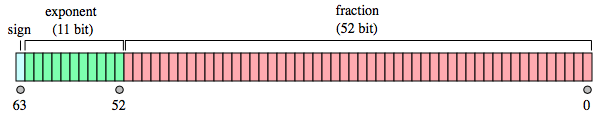
\includegraphics[scale=0.3]{pics/float-ieee}
			\end{figure}
		}
		\uncover<2->{
  		\begin{figure}
				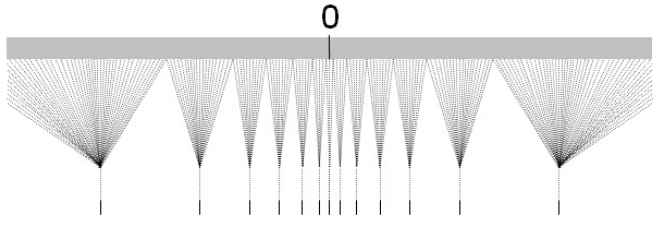
\includegraphics[scale=0.25]{pics/float-axis}
			\end{figure}
		}
		\uncover<3->{
			Beispiel:
			\begin{equation}
				A = \begin{pmatrix}
					10^{-20}	& 1 \\
					1					&	1
				\end{pmatrix} =
				\begin{pmatrix}
					1				&	0 \\
					10^{20}	&	1
				\end{pmatrix}
				\begin{pmatrix}
					10^{-20}	&	1 \\
					0					&	1-10^{20}
				\end{pmatrix}
			\end{equation}
		}
\end{frame}
%----------------------------end frame--------------------------------
\subsection{Begriffe}
%----------------------------begin frame------------------------------
\begin{frame}[fragile]
  \frametitle{Man erntet was man sät}
	\begin{itemize}

	\item \uncover<1->{
		Kondition ist Empfindlichkeit des Ergebnisses auf Störungen der Daten
	}
	\vspace*{1em}
	\uncover<3->{
		Konditionszahl: $\kappa = ^{||A||}/_{||A^{-1}||}$ \uncover<4->{, Matlab Beispiel: $\epsilon < ^1/_{cond(A)}$} \uncover<5->{, keine Brauchbare Lösung bei $\epsilon * cond(A) \sim 1$}
	}
	\vspace*{1em}
	\item \uncover<2->{
		Stabilität ist Empfindlichkeit des Algorihtmus auf Störungen der Daten
	}
	\vspace*{1em}
	\uncover<6->{
		Wachstumsfaktor: $\rho_{n} = ^{\max\limits_{i,j}{r_{i,j}}}/_{\max\limits_{i,j}{a_{i,j}}}$ \uncover<7->{, es macht Sinn eine Warnung auszugeben, falls der Faktor zu groß wird}
	}
	\end{itemize}
\end{frame}
%----------------------------end frame--------------------------------





\section{Suchverfahren}
\subsection{Partielle Pivotsuche}
%----------------------------begin frame------------------------------
\begin{frame}
  \frametitle{Algorithmus zur partiellen Pivotsuche}

  \setcounter{algorithm}{0} % sonst haben wir auf jeder Folie einen
                            % neuen Algorithmus :)
  \begin{algorithm}[H]
  \caption{Partielle Pivotisierung%
    \label{alg:partial_pivoting}}
  \begin{algorithmic}[1]

		% Ein- und Ausgabe
		\REQUIRE $\bfA\in\mathbb{R}^{m\times n}$ mit $\Rang(\bfA)=n$, $\bfP\in\mathbb{R}^{n\times n}$.
		\ENSURE $\bfL\in\mathbb{R}^{m\times n}$ untere Dreiecksmatrix, $\bfR\in\mathbb{R}^{n\times n}$ obere Dreiecksmatrix.

		% Initialisierung
		\STATE \alert<2>{$[m,n] \leftarrow \textsf{size}(\bfA)$;}
		\STATE \alert<3>{$\bfR \leftarrow \bfA$,} \alert<4>{$\bfL \leftarrow \bfP \leftarrow \textsf{eye}(m,n)$;}

		% Schleife
		\FOR{$k = 1:n-1$}

			% Finde betragsmäßig maximales Element
			\STATE \alert<5>{$[a_{max},i_{max}] \leftarrow \max\limits_{k \leq i \leq n}\{|a_{i,k}|\}$}

			% Zeilenaustausch
			\IF{$i_{max} \neq k$}
				\STATE \alert<6>{$\bfP([k\textsf{ }i_{max}],:) \leftarrow \bfP([i_{max}\textsf{ }k],:)$}
			\ENDIF

			% Berechnung der Koeffizienten-Spalte in der L-Matrix
			\STATE \alert<7>{$\bfL(k+1:n,k) \leftarrow \bfR(k+1:n,k)/a_{max}$}

			% Berechnung der Zeile in der R-Matrix
			\STATE \alert<8>{$\bfR(k+1:n,k:n) \leftarrow \bfR(k+1:n,k:n) - \bfL(k+1:n,k:n).*\bfR(k:n,k:n)$}

		\ENDFOR
  \end{algorithmic}
\end{algorithm}

\end{frame}
%----------------------------end frame--------------------------------
%----------------------------begin frame------------------------------
\begin{frame}
  \frametitle{Beispiel zur partiellen Pivotsuche}
  \label{ex:partial_pivoting}
  \begin{columns}[onlytextwidth]
    \column{.2\textwidth}
    \uncover<1->{%
      \tikz[baseline=1pt,scale=1]{%
        \matrix [matrix of math nodes, ampersand replacement=\&] (m) {%
                \& q_1 \& q_2 \& q_3 \\
            p_1 \& \alert<2,3,4>{0}   \& 2   \& \llap{$-$}3  \\
            p_2 \& \alert<4>{2}   \& 2   \& 1   \\
            p_3 \& 2   \& 4   \& 4   \\
        };
        \only<3,4>{%
          \draw[black] (m-2-2.north west) -- (m-2-2.north east) -- (m-4-2.south east) -- (m-4-2.south west) -- (m-2-2.north west);
        }
      }
    }%
    \column{.2\textwidth}
    \uncover<5->{%
      \tikz[baseline=1pt,scale=1]{%
        \matrix [matrix of math nodes, ampersand replacement=\&] (m) {%
                \& q_1 \& q_2 \& q_3	\\
            \alert<5>{p_2} \& \alert<6>{2}   \& 2   \& 1	\\
            \alert<5>{p_1} \& 0   \& 2   \& \llap{$-$}3		\\
            p_3 \& 2   \& 4   \& 4		\\
        };
      }
    }%
    \column{.2\textwidth}
    \uncover<7->{%
      \tikz[baseline=1pt,scale=1]{%
        \matrix [matrix of math nodes, ampersand replacement=\&] (m) {%
                \& q_1 \& q_2 \& q_3	\\
            p_2 \& 2   \& 2   \& 1		\\
            p_1 \& 0   \& \alert<8,9,10,11>{2}   \& \llap{$-$}3	\\
            p_3 \& 0   \& \alert<10>{2}   \& 3	\\
        };
        \only<9,10>{%
          \draw[black] (m-3-3.north west) -- (m-3-3.north east) -- (m-4-3.south east) -- (m-4-3.south west) -- (m-3-3.north west);
        }
      }
    }%
    \column{.2\textwidth}
    \uncover<12->{%
      \tikz[baseline=1pt,scale=1]{%
        \matrix [matrix of math nodes, ampersand replacement=\&] (m) {%
                \& q_1 \& q_2 \& q_3	\\
            p_2 \& 2   \& 2   \& 1		\\
            p_1 \& 0   \& 2   \& \llap{$-$}3	\\
            p_3 \& 0   \& 0   \& 6		\\
        };
      }
    }%
  \end{columns}
  \vspace*{1em}
  Matrizen, die Gleichung $\bf{PAQ}=\bf{LR}$ erfüllen:
  \begin{equation}
    P =
    \only<1-4>{%
      \begin{pmatrix}
        1 & 0 & 0 \\
        0 & 1 & 0 \\
        0 & 0 & 1 \\
      \end{pmatrix},
    }
    \only<5->{%
      \begin{pmatrix}
        \alert<5>{0} & \alert<5>{1} & \alert<5>{0} \\
        \alert<5>{1} & \alert<5>{0} & \alert<5>{0} \\
        0 & 0 & 1 \\
      \end{pmatrix},
    }
    Q = \begin{pmatrix}
      1 & 0 & 0 \\
      0 & 1 & 0 \\
      0 & 0 & 1 \\
    \end{pmatrix},
    L =
    \only<1-5>{%
      \begin{pmatrix}
        1 & 0 & 0 \\
        0 & 1 & 0 \\
        0 & 0 & 1 \\
      \end{pmatrix}
    }
    \only<6-10>{%
      \begin{pmatrix}
        1 & 0 & 0 \\
        \alert<6>{0} & 1 & 0 \\
        \alert<6>{1} & 0 & 1 \\
      \end{pmatrix}
    }
    \only<11->{%
      \begin{pmatrix}
        1 & 0 & 0 \\
        0 & 1 & 0 \\
        1 & \alert<11>{1} & 1 \\
      \end{pmatrix}
    }
  \end{equation}
\end{frame}
%----------------------------end frame--------------------------------
%----------------------------begin frame------------------------------
\begin{frame}[fragile]
	\frametitle{Eigenschaften der partiellen Pivotsuche}
	\begin{itemize}[<+->]
		\item Komplexität der Suche: $^{n^{2}}/_{2} \in O(n^2)$
		\vspace*{1em}
		\item Wachstumsfaktor: $\rho_{n}^{GEPP} \leq 2^{n-1}$, $n \geq 1$
		\vspace*{1em}
		\item Spezielle Matrizen:
		\vspace*{1em}
		\begin{itemize}[<+->]
			\item Diagonalmatrix und Tridiagonalmatrix: $\rho_{n}^{GEPP} \leq 2$
			\vspace*{1em}
			\item Hessenberg: $\rho_{n}^{GEPP} \leq n$
			\vspace*{1em}
			\item (n, n)-Bandmatrix: $\rho_{n}^{GEPP} \leq 2^{2n-1} - (n-1)2n^{p-2}$
			\vspace*{1em}
			\item SPD: $\rho_{n}^{GEPP} = 1$
			\end{itemize}
	\end{itemize}
\end{frame}
%----------------------------end frame--------------------------------





\subsection{Totale Pivotsuche}
%----------------------------begin frame------------------------------
\begin{frame}
  \frametitle{Algorithmus zur totalen Pivotsuche}

  \setcounter{algorithm}{0} % sonst haben wir auf jeder Folie einen
                            % neuen Algorithmus :)
  \begin{algorithm}[H]
  \caption{Totale Pivotisierung%
    \label{alg:total_pivoting}}
  \begin{algorithmic}[1]

		% Ein- und Ausgabe
		\REQUIRE $\bfA\in\mathbb{R}^{m\times n}$ mit $\Rang(\bfA)=n$, $\bfP\in\mathbb{R}^{n\times n}$, $\bfQ\in\mathbb{R}^{n\times n}$.
		\ENSURE $\bfL\in\mathbb{R}^{m\times n}$ untere Dreiecksmatrix, $\bfR\in\mathbb{R}^{n\times n}$ obere Dreiecksmatrix.

		% Initialisierung
		\STATE \alert<2>{$[m,n] \leftarrow \textsf{size}(\bfA)$;}
		\STATE \alert<3>{$\bfR \leftarrow \bfA$,} \alert<4>{$\bfL \leftarrow \bfP \leftarrow \bfQ \leftarrow \textsf{eye}(m,n)$;}

		% Schleife
		\FOR{$k = 1:n-1$}

			% Finde betragsmäßig maximales Element
			\STATE \alert<5>{$[a_{max},i_{max},j_{max}] \leftarrow \max\limits_{k \leq i \leq n, k \leq j \leq n}\{|a_{i,j}|\}$}

			% Zeilenaustausch
			\IF{$i_{max} \neq k$}
				\STATE \alert<6>{$\bfP([k\textsf{ }i_{max}],:) \leftarrow \bfP([i_{max}\textsf{ }k],:)$}
			\ENDIF

			% Spaltenaustausch
			\IF{$j_{max} \neq k$}
				\STATE \alert<7>{$\bfQ(:,[k\textsf{ }j_{max}]) \leftarrow \bfQ(:,[j_{max}\textsf{ }k])$}
			\ENDIF

			% Berechnung der Koeffizienten-Spalte in der L-Matrix
			\STATE \alert<8>{$\bfL(k+1:n,k) \leftarrow \bfR(k+1:n,k)/a_{max}$}

			% Berechnung der Zeile in der R-Matrix
			\STATE \alert<9>{$\bfR(k+1:n,k:n) \leftarrow \bfR(k+1:n,k:n) - \bfL(k+1:n,k:n).*\bfR(k:n,k:n)$}

		\ENDFOR
  \end{algorithmic}
\end{algorithm}

\end{frame}
%----------------------------end frame--------------------------------
%----------------------------begin frame------------------------------
\begin{frame}
  \frametitle{Beispiel zur totalen Pivotsuche}
  \label{ex:complete_pivoting}
  \begin{columns}[onlytextwidth]
    \column{.2\textwidth}
    \uncover<1->{%
      \tikz[baseline=1pt,scale=1]{%
        \matrix [matrix of math nodes, ampersand replacement=\&] (m) {%
                \& q_1 \& q_2 \& q_3 \\
            p_1 \& \alert<2,3,4>{0}   \& 2   \& \llap{$-$}3  \\
            p_2 \& 2   \& 2   \& 1   \\
            p_3 \& 2   \& \alert<4>{4}   \& 4   \\
        };
        \only<3,4>{%
          \draw[black] (m-2-2.north west) -- (m-2-4.north east) -- (m-4-4.south east) -- (m-4-2.south west) -- (m-2-2.north west);
        }
      }
    }%
    \column{.2\textwidth}
    \uncover<5->{%
      \tikz[baseline=1pt,scale=1]{%
        \matrix [matrix of math nodes, ampersand replacement=\&] (m) {%
                \& \alert<5>{q_2} \& \alert<5>{q_1} \& q_3 \\
            \alert<5>{p_3} \& \alert<6>{4}   \& 2   \& 4   \\
            p_2 \& 2   \& 2   \& 1  \\
            \alert<5>{p_1} \& 2   \& 0   \& \llap{$-$}3   \\
        };
      }
    }%
    \column{.2\textwidth}
    \uncover<7->{%
      \tikz[baseline=1pt,scale=1]{%
        \matrix [matrix of math nodes, ampersand replacement=\&] (m) {%
                \& q_2 \& q_1 \& q_3 \\
            p_3 \& 4   \& 2   \& 4  \\
            p_2 \& 0   \& \alert<8,9,10>{1}   \& \llap{$-$}1   \\
            p_1 \& 0   \& \llap{$-$}1   \& \alert<10>{\llap{$-$}5}   \\
        };
        \only<9,10>{%
          \draw[black] (m-3-3.north west) -- (m-3-4.north east) -- (m-4-4.south east) -- (m-4-3.south west) -- (m-3-3.north west);
        }
      }
    }%
    \column{.2\textwidth}
    \uncover<11->{%
      \tikz[baseline=1pt,scale=1]{%
        \matrix [matrix of math nodes, ampersand replacement=\&] (m) {%
                \& q_2 \& \alert<11>{q_3} \& \alert<11>{q_1}	\\
            p_3 \& 4   \& 2   \& 4	\\
            \alert<11>{p_1} \& 0   \& \alert<12>{\llap{$-$}5}   \& \llap{$-$}1   \\
            \alert<11>{p_2} \& 0   \& \llap{$-$}1   \& 1	\\
        };
      }
    }%
    \column{.2\textwidth}
    \uncover<13->{%
      \tikz[baseline=1pt,scale=1]{%
        \matrix [matrix of math nodes, ampersand replacement=\&] (m) {%
                \& q_2 \& q_3 \& q_1	\\
            p_3 \& 4   \& 2   \& 4		\\
            p_1 \& 0   \& \llap{$-$}5   \& \llap{$-$}1   \\
            p_2 \& 0   \& 0   \& 1^1/_5	\\
        };
      }
    }%
  \end{columns}
  \vspace*{1em}
  Matrizen, die Gleichung $\bf{PAQ}=\bf{LR}$ erfüllen:
  \begin{equation}
    P =
    \only<1-4>{%
      \begin{pmatrix}
        1 & 0 & 0 \\
        0 & 1 & 0 \\
        0 & 0 & 1 \\
      \end{pmatrix},
    }
    \only<5-10>{%
      \begin{pmatrix}
        \alert<5>{0} & \alert<5>{0} & \alert<5>{1} \\
        0 & 1 & 0 \\
        \alert<5>{1} & \alert<5>{0} & \alert<5>{0} \\
      \end{pmatrix},
    }
    \only<11->{%
      \begin{pmatrix}
        0 & 0 & 1 \\
        \alert<11>{1} & \alert<11>{0} & \alert<11>{0} \\
        \alert<11>{0} & \alert<11>{1} & \alert<11>{0} \\
      \end{pmatrix},
    }
    Q =
    \only<1-4>{%
      \begin{pmatrix}
        1 & 0 & 0 \\
        0 & 1 & 0 \\
        0 & 0 & 1 \\
      \end{pmatrix},
    }
    \only<5-10>{%
      \begin{pmatrix}
        \alert<5>{0} & \alert<5>{1} & 0 \\
        \alert<5>{1} & \alert<5>{0} & 0 \\
        \alert<5>{0} & \alert<5>{0} & 1 \\
      \end{pmatrix},
    }
    \only<11->{%
      \begin{pmatrix}
        0 & \alert<11>{0} & \alert<11>{1} \\
        1 & \alert<11>{0} & \alert<11>{0} \\
        0 & \alert<11>{1} & \alert<11>{0} \\
      \end{pmatrix},
    }
    L =
    \only<1-5>{%
      \begin{pmatrix}
        1 & 0 & 0 \\
        0 & 1 & 0 \\
        0 & 0 & 1 \\
      \end{pmatrix}
    }
    \only<6-11>{%
      \begin{pmatrix}
        1 & 0 & 0 \\
        \alert<6>{^1/_2} & 1 & 0 \\
        \alert<6>{^1/_2} & 0 & 1 \\
      \end{pmatrix}
    }
    \only<12->{%
      \begin{pmatrix}
        1 & 0 & 0 \\
        ^1/_2 & 1 & 0 \\
        ^1/_2 & \alert<12>{^1/_5} & 1 \\
      \end{pmatrix}
    }
  \end{equation}
\end{frame}
% ----------------------------end frame--------------------------------
%----------------------------begin frame------------------------------
\begin{frame}[fragile]
	\frametitle{Eigenschaften der totalen Pivotsuche}
	\begin{itemize}[<+->]
		\item Komplexität der Suche: $^{n^{3}}/_{3} \in O(n^3)$
		\vspace*{1em}
		\item Wachstumsfaktor: $\rho_{n}^{GETP} \leq 2\sqrt{n}n^{ln(n)/4}$, $n \geq 1$
		% \vspace*{1em}
		% \item Warum extra Umstände?
	\end{itemize}
\end{frame}
%----------------------------end frame--------------------------------





\subsection{Rook-Pivotsuche}
%----------------------------begin frame------------------------------
\begin{frame}[shrink=12]
  \frametitle{Algorithmus zur Rook-Pivotsuche}
  \setcounter{algorithm}{0} % sonst haben wir auf jeder Folie einen
                            % neuen Algorithmus :)
  \begin{algorithm}[H]
  \caption{Rook Pivotisierung%
    \label{alg:rook_pivoting}}
  \begin{algorithmic}[1]

		% Ein- und Ausgabe
		\REQUIRE $\bfA\in\mathbb{R}^{m\times n}$ mit $\Rang(\bfA)=n$, $\bfP\in\mathbb{R}^{n\times n}$, $\bfP\in\mathbb{R}^{n\times n}$.
		\ENSURE $\bfL\in\mathbb{R}^{m\times n}$ untere Dreiecksmatrix, $\bfR\in\mathbb{R}^{n\times n}$ obere Dreiecksmatrix.
  	% COMMENT , $\bf{PA}=\bf{LR}$.

		% Initialisierung
		\STATE \alert<2>{$[m,n] \leftarrow \textsf{size}(\bfA)$;}
		\STATE \alert<3>{$\bfR \leftarrow \bfA$,} \alert<4>{$\bfL \leftarrow \bfP \leftarrow \textsf{eye}(m,n)$;}

		% Schleife
		\FOR{$k = 1:n-1$}

			% Finde betragsmäßig maximales Element
			\STATE \alert<5>{$a_{max} \leftarrow a_{kk}$, $[a_{col}, i_{max}] \leftarrow \max\limits_{k \leq i \leq n}\{|a_{i,k}\}|$, $a_{row} \leftarrow it \leftarrow 0$}
			\WHILE{$a_{max} < a_{col}$ \OR $a_{max} < a_{row}$}
				\STATE \alert<6>{$a_{max} \leftarrow \max\{a_{row}, a_{col}\}$}
				\IF{$it$ is odd}
				\STATE \alert<7>{$[a_{col}, i_{max}] \leftarrow \max\limits_{k \leq i \leq n}\{|a_{i,j_{max}}|\}$}
				\ELSE
				\STATE \alert<8>{$[a_{row}, j_{max}] \leftarrow \max\limits_{k \leq j \leq n}\{|a_{i_{max},j}|\}$}
				\ENDIF
				\STATE \alert<9>{$it++$;}
			\ENDWHILE

			\STATE \alert<10>{$a_{max} \leftarrow \max\{a_{row}, a_{col}\}$}

			% Zeilenaustausch
			\IF{$i_{max} \neq k$}
				\STATE \alert<11>{$\bfP([k\textsf{ }i_{max}],:) \leftarrow \bfP([i_{max}\textsf{ }k],:)$}
			\ENDIF
			% Spaltenaustausch
			\IF{$j_{max} \neq k$}
				\STATE \alert<12>{$\bfQ(:,[k\textsf{ }j_{max}]) \leftarrow \bfQ(:,[j_{max}\textsf{ }k])$}
			\ENDIF

			% Berechnung der Koeffizienten-Spalte in der L-Matrix
			\STATE \alert<13>{$\bfL(k+1:n,k) \leftarrow \bfR(k+1:n,k)/a_{max}$}

			% Berechnung der Zeile in der R-Matrix
			\STATE \alert<14>{$\bfR(k+1:n,k:n) \leftarrow \bfR(k+1:n,k:n) - \bfL(k+1:n,k:n).*\bfR(k:n,k:n)$}

		\ENDFOR
  \end{algorithmic}
\end{algorithm}

\end{frame}
%----------------------------end frame--------------------------------
%----------------------------begin frame------------------------------
\begin{frame}
  \frametitle{Beispiel zur Rook-Pivotsuche}
	\label{ex:rook_pivoting}
  \begin{columns}[onlytextwidth]
    \column{.2\textwidth}
    \uncover<1->{%
      \tikz[baseline=1pt,scale=1]{%
        \matrix [matrix of math nodes, ampersand replacement=\&] (m) {%
                \& q_1 \& q_2 \& q_3 \\
            p_1 \& \alert<2,3,4>{0}   \& 2   \& \llap{$-$}3  \\
            p_2 \& \alert<4,5,6>{2}   \& \alert<6>{2}   \& 1   \\
            p_3 \& 2   \& 4   \& 4   \\
        };
        \only<3,4>{%
          \draw[black] (m-2-2.north west) -- (m-2-2.north east) -- (m-4-2.south east) -- (m-4-2.south west) -- (m-2-2.north west);
        }
        \only<5,6>{%
          \draw[black] (m-3-2.north west) -- (m-3-4.north east) -- (m-3-4.south east) -- (m-3-2.south west) -- (m-3-2.north west);
        }
      }
    }%
    \column{.2\textwidth}
    \uncover<7->{%
      \tikz[baseline=1pt,scale=1]{%
        \matrix [matrix of math nodes, ampersand replacement=\&] (m) {%
                \& q_1 \& q_2 \& q_3 \\
            \alert<7>{p_2} \& \alert<8>{2}   \& 2   \& 1   \\
            \alert<7>{p_1} \& 0   \& 2   \& \llap{$-$}3  \\
            p_3 \& 2   \& 4   \& 4   \\
        };
      }
    }%
    \column{.2\textwidth}
    \uncover<9->{%
      \tikz[baseline=1pt,scale=1]{%
        \matrix [matrix of math nodes, ampersand replacement=\&] (m) {%
                \& q_1 \& q_2 \& q_3 \\
            p_2 \& 2   \& 2   \& 1  \\
            p_1 \& 0   \& \alert<10-14>{2}   \& \alert<14-16>{\llap{$-$}3}   \\
            p_3 \& 0   \& \alert<12>{2}   \& \alert<16>{3}   \\
        };
        \only<11,12>{%
          \draw[black] (m-3-3.north west) -- (m-3-3.north east) -- (m-4-3.south east) -- (m-4-3.south west) -- (m-3-3.north west);
        }
        \only<13-14>{%
          \draw[black] (m-3-3.north west) -- (m-3-4.north east) -- (m-3-4.south east) -- (m-3-3.south west) -- (m-3-3.north west);
        }
        \only<15,16>{%
          \draw[black] (m-3-4.north west) -- (m-3-4.north east) -- (m-4-4.south east) -- (m-4-4.south west) -- (m-3-4.north west);
        }
      }
    }%
    \column{.2\textwidth}
    \uncover<17->{%
      \tikz[baseline=1pt,scale=1]{%
        \matrix [matrix of math nodes, ampersand replacement=\&] (m) {%
                \& q_1 \& \alert<17>{q_3} \& \alert<17>{q_2} \\
            p_2 \& 2   \& 1   \& 2  \\
            p_1 \& 0   \& \alert<18>{\llap{$-$}3}   \& 2   \\
            p_3 \& 0   \& 3   \& 2   \\
        };
      }
    }%
    \column{.2\textwidth}
    \uncover<19->{%
      \tikz[baseline=1pt,scale=1]{%
        \matrix [matrix of math nodes, ampersand replacement=\&] (m) {%
                \& q_1 \& q_3 \& q_2 \\
            p_2 \& 2   \& 1   \& 2  \\
            p_1 \& 0   \& \llap{$-$}3   \& 2   \\
            p_3 \& 0   \& 0   \& 4   \\
        };
      }
    }%
  \end{columns}
  \vspace*{1em}
  Matrizen, die Gleichung $\bf{PAQ}=\bf{LR}$ erfüllen:
  \begin{equation}
    P =
    \only<1-6>{%
      \begin{pmatrix}
        1 & 0 & 0 \\
        0 & 1 & 0 \\
        0 & 0 & 1 \\
      \end{pmatrix},
    }
    \only<7->{%
      \begin{pmatrix}
        \alert<7>{0} & \alert<7>{1} & \alert<7>{0} \\
        \alert<7>{1} & \alert<7>{0} & \alert<7>{0} \\
        0 & 0 & 1 \\
      \end{pmatrix},
    }
    Q =
    \only<1-16>{%
      \begin{pmatrix}
        1 & 0 & 0 \\
        0 & 1 & 0 \\
        0 & 0 & 1 \\
      \end{pmatrix},
    }
    \only<17->{%
      \begin{pmatrix}
        1 & \alert<17>{0} & \alert<17>{0} \\
        0 & \alert<17>{0} & \alert<17>{1} \\
        0 & \alert<17>{1} & \alert<17>{0} \\
      \end{pmatrix},
    }
    L =
    \only<1-7>{%
      \begin{pmatrix}
        1 & 0 & 0 \\
        0 & 1 & 0 \\
        0 & 0 & 1 \\
      \end{pmatrix}
    }
    \only<8-17>{%
      \begin{pmatrix}
        1 & 0 & 0 \\
        \alert<8>{0} & 1 & 0 \\
        \alert<8>{1} & 0 & 1 \\
      \end{pmatrix}
    }
    \only<18->{%
      \begin{pmatrix}
        1 & 0 & 0 \\
        0 & 1 & 0 \\
        1 & \alert<18>{\llap{$-$}1} & 1 \\
      \end{pmatrix}
    }
  \end{equation}
\end{frame}
% ----------------------------end frame--------------------------------
%----------------------------begin frame------------------------------
\begin{frame}[fragile]
	\frametitle{Eigenschaften der Rook-Pivotsuche}
	\begin{itemize}[<+->]
		\item Komplexität der Suche: $^{3n^{2}}/_{2} \in O(n^2)$
		\vspace*{1em}
		\item Wachstumsfaktor: $\rho_{n}^{GERP} \leq 1.5n^{3ln(n)/4}$, $n \geq 1$
		% \vspace*{1em}
		% \item Warum extra Umstände?
	\end{itemize}
\end{frame}
%----------------------------end frame--------------------------------





\section{Fazit}
%----------------------------begin frame------------------------------
\begin{frame}
  \frametitle{Fazit \& Ausblick}

  Fazit:

	\vspace*{1em}

  \begin{itemize}
  \item Stets die Rechnereinschränkungen beachten.
  \vspace*{1em}
	\item Meistens reicht die einfachere Methode aus.
  \vspace*{1em}
  \end{itemize}


\end{frame}
%----------------------------end frame--------------------------------
\appendix
\backupbegin
%----------------------------begin frame------------------------------
\begin{frame}
  \frametitle{Dankeschön!}

\selectlanguage{ngerman}

  \Large
  \begin{center}
    Vielen Dank für die Aufmerksamkeit!

    \vspace*{3em}

    \uncover<2->{(Möge der Vortrag von Andrej besser sein.)}
  \end{center}

\end{frame}
%----------------------------begin frame------------------------------
\begin{frame}
  \frametitle{Literatur}
	Watkins, David S.: Fundamentals of matrix computations, Wiley-Interscience [John Wiley \& Sons], New York, 2002 \\
	\vspace*{1em}
	Jens-Peter M. Zemke: Numerische Mathematik, ausgewählte Vertiefungen - ein Vorlesungsskript, 3. Februar 2014 \\
	\vspace*{1em}
	http://www.math.sjsu.edu/~foster/m143m/pivoting\_examples\_2.pdf (Stand: 15. Mai 2017) \\
	\vspace*{1em}
	https://www.tu-chemnitz.de/mathematik/numa/lehre/numerik-2015/Folien/numerik2.pdf \\
	\vspace*{1em}
	https://www.tu-chemnitz.de/mathematik/numa/lehre/numerik-2015/Folien/numerik3.pdf
	% \bibliography{Proseminar}
	% \bibliographystyle{apalike}

\end{frame}
%----------------------------end frame--------------------------------
\backupend

\end{document}

%%% Local Variables:
%%% mode: latex
%%% TeX-master: t
%%% End:
